\documentclass[tikz,border=8pt]{standalone}

\usepackage[T1]{fontenc}
\usepackage{lmodern}
\usetikzlibrary{arrows.meta,backgrounds,calc,positioning,fit,shapes.geometric}

\definecolor{flowblue}{HTML}{0072B2}
\definecolor{flowgreen}{HTML}{009E73}
\definecolor{flowbrown}{HTML}{8C564B}
\definecolor{flowpurple}{HTML}{6F4EA1}
\definecolor{floworange}{HTML}{D55E00}
\definecolor{ink}{HTML}{243447}
\definecolor{mutedink}{HTML}{52606D}
\definecolor{linegray}{HTML}{9AA5B1}
\definecolor{panel}{HTML}{F5F7FA}
\definecolor{ownedfill}{HTML}{E8F1F8}
\definecolor{storefill}{HTML}{FFF1CC}
\definecolor{externalfill}{HTML}{F3ECF8}

\tikzset{
  box/.style={
    draw=linegray,
    fill=white,
    rounded corners=2pt,
    line width=0.6pt,
    minimum height=10mm,
    text width=30mm,
    align=center,
    font=\sffamily\small,
    text=ink,
    inner sep=4pt
  },
  actor/.style={box,text width=24mm},
  component/.style={box,fill=ownedfill},
  store/.style={box,fill=storefill,text width=24mm},
  external/.style={box,fill=externalfill,text width=34mm},
  network/.style={box,text width=26mm},
  boundary title/.style={font=\sffamily\bfseries\large,text=ink,anchor=west},
  flow/.style={-{Latex[length=3mm,width=2.2mm]},line width=1.6pt},
  story one/.style={flow,draw=flowblue},
  story two/.style={flow,draw=flowgreen},
  story three/.style={flow,draw=flowbrown},
  story four/.style={flow,draw=flowpurple},
  story five/.style={flow,draw=floworange},
  relation/.style={draw=linegray,line width=1.1pt},
  edge label/.style={
    fill=none,
    inner xsep=1.5pt,
    inner ysep=3pt,
    font=\sffamily\scriptsize,
    text=mutedink,
    align=center
  },
  every node/.append style={font=\sffamily}
}

\newcommand{\storyStep}[2]{%
  \tikz[baseline=(step.base)]
    \node[circle,fill=#1,text=white,inner sep=1.1pt,
      font=\sffamily\bfseries\tiny] (step) {#2};%
}


\tikzset{
  dependency/.style={relation,-{Latex[length=2.3mm,width=1.6mm]}},
  planned/.style={component,dashed,fill=white},
  smallbox/.style={component,text width=27mm,minimum height=10mm},
  table/.style={box,align=left,text width=50mm,inner sep=7pt,font=\sffamily\small},
  fk/.style={relation,-{Latex[length=2.6mm]},draw=ink,line width=1.2pt},
  logical/.style={relation,-{Latex[length=2.6mm]},draw=flowblue,dashed,line width=1.2pt},
  note/.style={font=\sffamily\small,text=mutedink,align=left},
  title/.style={font=\sffamily\bfseries\Large,text=ink,anchor=west}
}

\begin{document}
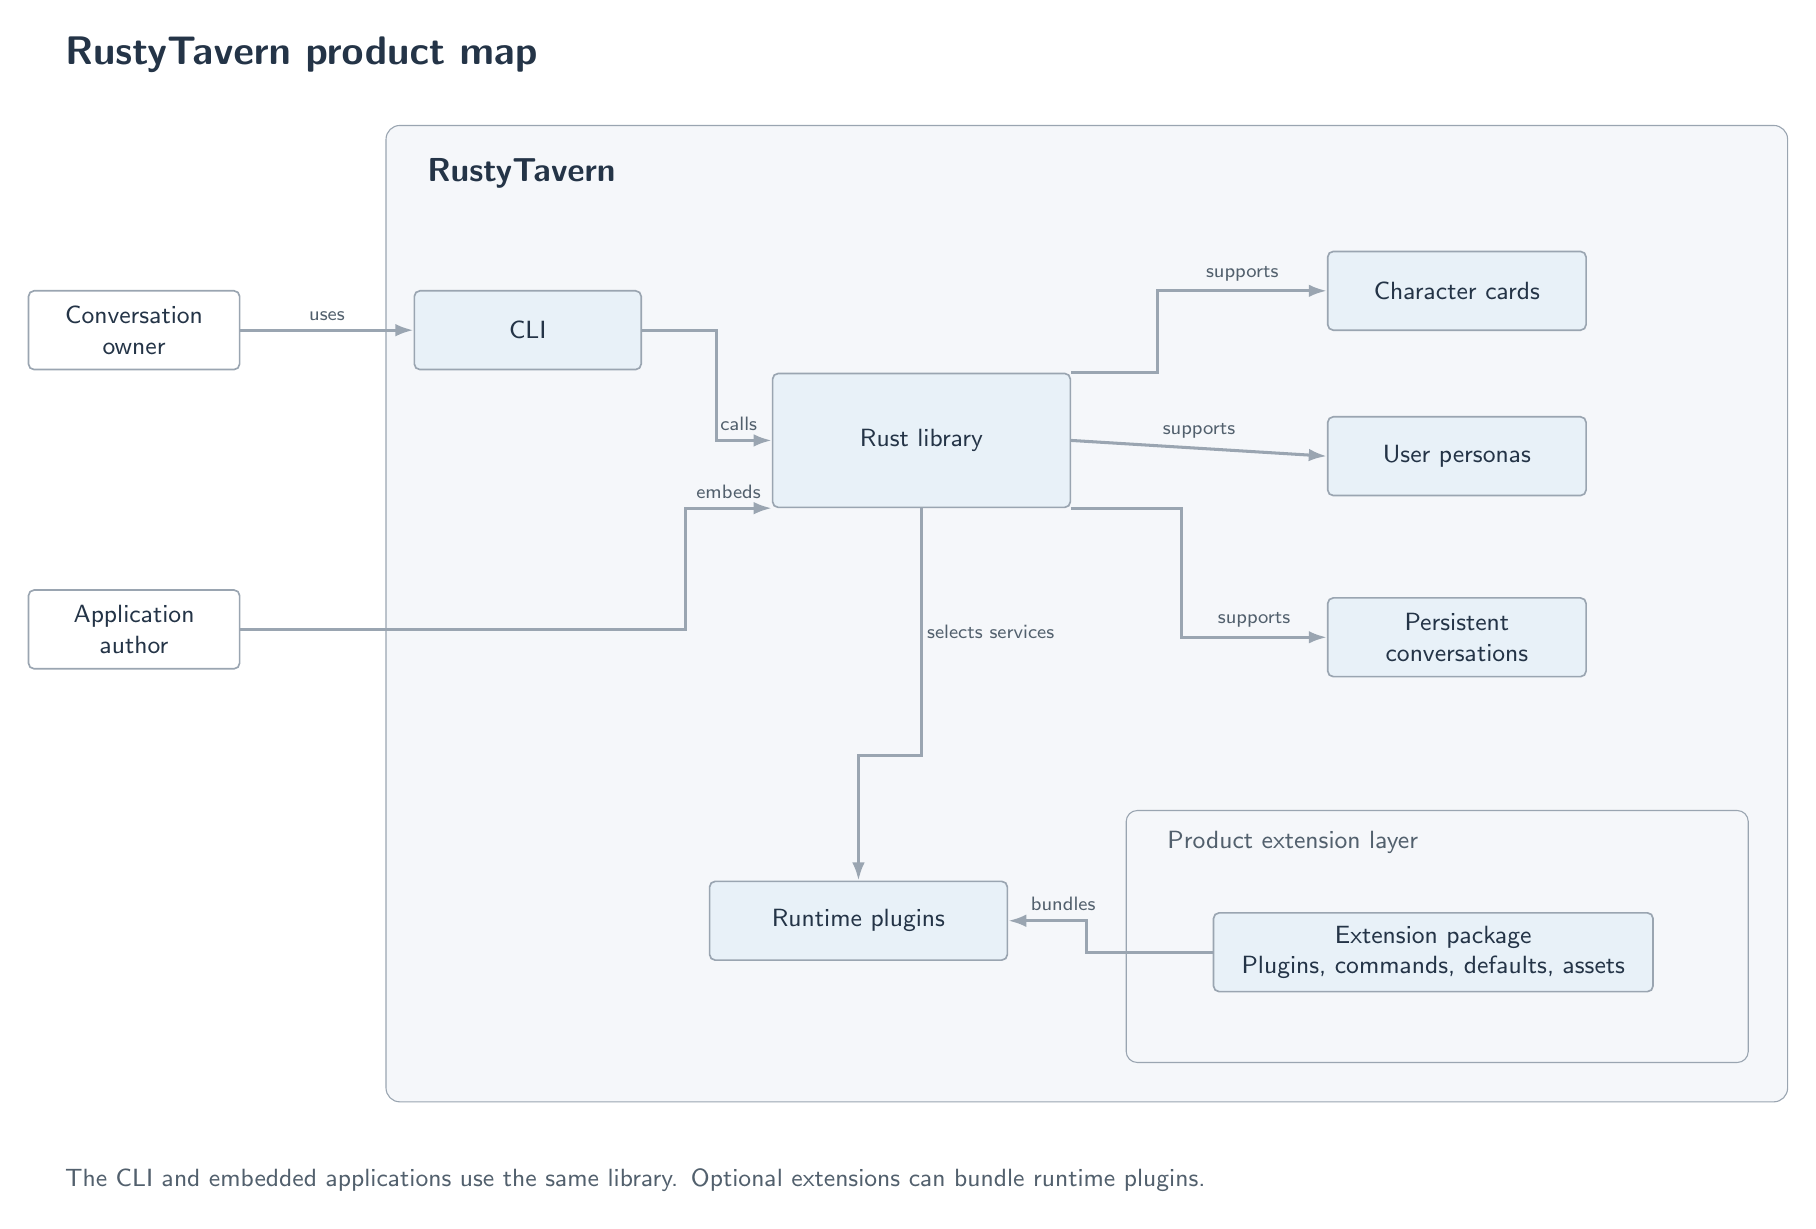
\begin{tikzpicture}[x=1cm,y=1cm]

\node[title] at (-1,13.2) {RustyTavern product map};
\begin{scope}[on background layer]
  \filldraw[fill=panel,draw=linegray,rounded corners=5pt] (3.2,-0.1) rectangle (21,12.3);
  \draw[linegray,rounded corners=4pt] (12.6,0.4) rectangle (20.5,3.6);
\end{scope}
\node[boundary title] at (3.6,11.7) {RustyTavern};
\node[note,anchor=west] at (13,3.2) {Product extension layer};
\node[actor] (person) at (0,9.7) {Conversation\\owner};
\node[actor] (author) at (0,5.9) {Application\\author};
\node[component,text width=26mm] (cli) at (5,9.7) {CLI};
\node[component,text width=35mm,minimum height=17mm] (lib) at (10,8.3) {Rust library};
\node[component] (cards) at (16.8,10.2) {Character cards};
\node[component] (persona) at (16.8,8.1) {User personas};
\node[component] (sessions) at (16.8,5.8) {Persistent\\conversations};
\node[component,text width=35mm] (plugins) at (9.2,2.2) {Runtime plugins};
\node[component,text width=53mm] (extension) at (16.5,1.8) {Extension package\\Plugins, commands, defaults, assets};
\draw[dependency] (person.east) -- node[edge label,above] {uses} (cli.west);
\draw[dependency] (cli.east) -- (7.4,9.7) |- node[edge label,pos=.7,above] {calls} (lib.west);
\draw[dependency] (author.east) -- (7,5.9) |- node[edge label,pos=.75,above] {embeds} (lib.south west);
\draw[dependency] (lib.north east) -| (13,9.3) |- node[edge label,pos=.75,above] {supports} (cards.west);
\draw[dependency] (lib.east) -- node[edge label,above] {supports} (persona.west);
\draw[dependency] (lib.south east) -| (13.3,7.3) |- node[edge label,pos=.75,above] {supports} (sessions.west);
\draw[dependency] (lib.south) -- node[edge label,right] {selects services} (10,4.3) -| (plugins.north);
\draw[dependency] (extension.west) -- (12.1,1.8) |- node[edge label,pos=.65,above] {bundles} (plugins.east);
\node[note,anchor=west,text width=210mm] at (-1,-1.1) {The CLI and embedded applications use the same library. Optional extensions can bundle runtime plugins.};

\end{tikzpicture}
\end{document}
